\documentclass[11pt]{article}

\usepackage[utf8]{inputenc}
\usepackage[T1]{fontenc}
\usepackage{amsmath,amssymb,amsthm}
\usepackage{mathtools}
\usepackage{algorithm}
\usepackage{algpseudocode}
\usepackage{booktabs}
\usepackage{graphicx}
\usepackage{hyperref}
\usepackage{xcolor}
\usepackage{listings}
\usepackage[margin=1in]{geometry}
\usepackage{enumitem}
\usepackage{tikz}
\usetikzlibrary{arrows.meta,positioning,shapes.geometric,fit,calc}
\usepackage{multirow}
\usepackage{caption}
\usepackage{subcaption}

\newtheorem{theorem}{Theorem}
\newtheorem{lemma}[theorem]{Lemma}
\newtheorem{definition}[theorem]{Definition}
\newtheorem{proposition}[theorem]{Proposition}
\newtheorem{corollary}[theorem]{Corollary}
\newtheorem{remark}[theorem]{Remark}
\newtheorem{example}[theorem]{Example}

\newcommand{\Set}{\mathbf{Set}}
\newcommand{\Pow}{\mathcal{P}}
\newcommand{\Fair}{\ensuremath{\mathrm{Fair}}}
\newcommand{\Act}{\ensuremath{\mathrm{Act}}}
\newcommand{\AP}{\ensuremath{\mathrm{AP}}}
\newcommand{\WF}{\ensuremath{\mathrm{WF}}}
\newcommand{\SF}{\ensuremath{\mathrm{SF}}}
\newcommand{\TFair}{$T$-Fair}
\newcommand{\CoaCert}{\textsc{CoaCert-TLA}}
\newcommand{\TLAplus}{TLA\textsuperscript{+}}
\newcommand{\naturals}{\mathbb{N}}
\newcommand{\reals}{\mathbb{R}}
\newcommand{\diam}{\ensuremath{\mathrm{diam}}}
\newcommand{\FPR}{\ensuremath{\mathrm{FPR}}}
\newcommand{\Streett}{\ensuremath{\mathrm{Streett}}}

\lstset{
  basicstyle=\ttfamily\small,
  keywordstyle=\bfseries\color{blue!70!black},
  commentstyle=\itshape\color{gray},
  stringstyle=\color{red!60!black},
  frame=single,
  breaklines=true,
  columns=flexible,
}

\title{\CoaCert{}: Witness-Certified Coalgebraic Compression\\for Finite-Domain \TLAplus{} Model Checking}

\date{}

\begin{document}

\maketitle

%% ============================================================
%% ABSTRACT
%% ============================================================
\begin{abstract}
We present \CoaCert{}, a tool that compresses \TLAplus{} state spaces via
coalgebraic bisimulation quotienting and emits Merkle-hashed witnesses
enabling independent verification of the reduction's correctness.
The theoretical foundation is a new endofunctor
$F(X) = \Pow(\AP) \times \Pow(X)^{\Act} \times \Fair(X)$
on $\Set$ whose coalgebra morphisms capture stuttering bisimulations
respecting weak and strong fairness constraints native to \TLAplus{}.
We prove a \emph{\TFair{} coherence theorem}---a distributive law
$\delta : T \circ \Fair \Rightarrow \Fair \circ T$ between the
stutter-closure monad~$T$ and the fairness component---and show this
coherence is necessary and sufficient for $F$-bisimulations to preserve
Streett acceptance conditions.
Building on this, we establish CTL$^*$$\setminus$X safety preservation
and Streett liveness preservation for the quotient, and prove W-method
completeness for conformance testing at depth
$k = \diam(H) + (m - n + 1)$.
On four benchmark families---Two-Phase Commit, Peterson's mutual
exclusion, Token Ring, and Dining Philosophers---\CoaCert{} achieves
compression ratios from $1.0\times$ (Token Ring, where each state is
structurally unique) to $64.0\times$ (Two-Phase Commit with 6 resource
managers, reducing 12{,}288 states to 192).
Comparison against a Paige--Tarjan partition-refinement baseline shows
that \CoaCert{} achieves identical quotient sizes while additionally
producing certified witnesses; the time overhead reflects the cost of
witness generation.
\end{abstract}

%% ============================================================
%% 1. INTRODUCTION
%% ============================================================
\section{Introduction}
\label{sec:intro}

The state explosion problem remains the central barrier to practical model
checking of distributed protocols specified in \TLAplus{}~\cite{Lamport02}.
TLC, Lamport's explicit-state checker~\cite{TLC}, exhaustively enumerates
every reachable state; for Two-Phase Commit with six resource managers this
yields 12{,}288 states, growing exponentially as participants are added.
Apalache's symbolic approach~\cite{Apalache} trades enumeration for SMT
encoding but encounters solver limits on the same protocols.
Critically, neither tool produces any independently inspectable
artifact---a user must trust the tool's implementation, its runtime, and
the machine it ran on.

The absence of certificates is not merely aesthetic.
In safety-critical domains---aerospace control protocols, financial
settlement systems, medical device firmware---regulatory bodies increasingly
demand evidence beyond ``the tool reported success.''
Certified model checking~\cite{Namjoshi01} addresses this by requiring the
checker to emit a proof certificate that a lightweight verifier can
independently validate.
However, existing certified approaches target specific logics and algorithms,
and none address state-space compression with fairness preservation.

\CoaCert{} addresses both problems simultaneously.
The key insight is that Lamport's \emph{stuttering equivalence}---the
semantic backbone of \TLAplus{} refinement mappings~\cite{Lamport94}---is
a coalgebraic bisimulation for a specific endofunctor on the category of
fair transition systems.
We define this functor, prove the \TFair{} coherence condition enabling
liveness preservation, instantiate $L^*$-style coalgebraic
learning~\cite{BarloccoKR19} to compute the minimal bisimulation quotient,
and emit a Merkle-hashed witness certifying the result.

\paragraph{Contributions.}
This paper makes the following contributions:
\begin{enumerate}[nosep]
\item \textbf{\TFair{} Coherence Theorem.}
  We define the stuttering-fair functor
  $F(X) = \Pow(\AP) \times \Pow(X)^{\Act} \times \Fair(X)$
  and prove that the stutter-closure monad~$T$ distributes over $\Fair$
  via a natural transformation
  $\delta : T \circ \Fair \Rightarrow \Fair \circ T$,
  with a constructive proof by exhaustion over saturation conditions
  (Section~\ref{sec:functor}).

\item \textbf{Preservation Theorems.}
  We prove that $F$-bisimulation quotients preserve CTL$^*$$\setminus$X
  properties (safety) and Streett acceptance conditions (liveness under
  fairness), extending the Browne--Clarke--Gr\"umberg result with the
  coherence condition (Section~\ref{sec:preservation}).

\item \textbf{Conformance Soundness.}
  We establish W-method completeness for bounded conformance testing at
  depth $k = \diam(H) + (m - n + 1)$ and design an incremental deepening
  protocol with convergence certificates
  (Section~\ref{sec:conformance}).

\item \textbf{Implementation and Evaluation.}
  An end-to-end implementation with empirical evaluation on four
  benchmark families showing compression ratios up to $64.0\times$,
  with certified witnesses verified independently.
  Honest comparison against a Paige--Tarjan baseline demonstrates
  identical quotient sizes with witness-generation overhead as the cost
  of certification (Sections~\ref{sec:architecture}--\ref{sec:evaluation}).
\end{enumerate}

%% ============================================================
%% 2. BACKGROUND
%% ============================================================
\section{Background}
\label{sec:background}

\subsection{\TLAplus{} Model Checking}

\TLAplus{}~\cite{Lamport02} specifies systems as state machines with an
initial-state predicate $\mathit{Init}$, a next-state relation
$\mathit{Next}$, and fairness constraints $\WF_v(A)$ (weak fairness) and
$\SF_v(A)$ (strong fairness).
TLC~\cite{TLC} performs explicit-state model checking by enumerating all
reachable states.
Properties are expressed in a stuttering-invariant fragment of temporal
logic: safety as invariants $\Box P$ and liveness under fairness as
$P \leadsto Q$.
The semantics of refinement is stuttering equivalence~\cite{Lamport94}:
a specification $S$ refines $T$ if every behavior of $S$ is, up to
stuttering, a behavior of $T$.

The \emph{state explosion problem} arises because the number of reachable
states grows exponentially in concurrent components.
For a protocol with $n$ participants each having $k$ local states, the
global state space may contain up to $k^n$ states.
Symmetry reduction~\cite{IpD96} and partial-order reduction~\cite{Peled93}
mitigate this in special cases but require manual annotations.

\paragraph{TLA-lite.}
\CoaCert{} operates on \emph{TLA-lite}, a finite-domain fragment of
\TLAplus{} supporting: finite-domain integers and booleans; finite sets
and functions; bounded sequences; primed variables and \texttt{UNCHANGED};
quantification over finite domains; and temporal operators including
$\Box[\mathit{Action}]_v$, $\WF_v(A)$, and $\SF_v(A)$.
This fragment covers standard distributed protocol benchmarks that TLC
can check with finite model values.

\subsection{Coalgebra and Bisimulation}

A \emph{coalgebra} for an endofunctor $F : \Set \to \Set$ is a pair
$(X, \gamma : X \to F(X))$ where $X$ is a set of states and $\gamma$
assigns to each state its one-step behavior~\cite{Rutten00}.
An \emph{$F$-bisimulation} between coalgebras $(X, \gamma)$ and
$(Y, \delta)$ is a relation $R \subseteq X \times Y$ such that related
states have $F$-related successors.
Two states are bisimilar if and only if they are identified by some
coalgebra morphism into a common quotient.

For labeled transition systems, the functor
$F(X) = \Pow(\AP) \times \Pow(X)^{\Act}$ yields standard Kripke-structure
bisimulation.
Beohar and K\"upper~\cite{BeoharK17} extended this to \emph{stuttering
bisimulation} by introducing a stutter-closure monad~$T$ that adjoins
stuttering-equivalent paths.

\begin{definition}[Stutter-Closure Monad]
\label{def:stutter-monad}
The stutter-closure monad $T : \Set \to \Set$ is defined on objects by
$T(X) = X^+$ (non-empty finite sequences over $X$) quotiented by the
equivalence that identifies sequences differing only in consecutive
repetitions.
The unit $\eta_X : X \to T(X)$ maps $x$ to $[x]$.
The multiplication $\mu_X : T(T(X)) \to T(X)$ flattens nested sequences.
\end{definition}

\subsection{Streett Acceptance Conditions}

Fairness in \TLAplus{} corresponds to \emph{Streett acceptance
conditions}~\cite{Streett82} on infinite paths.

\begin{definition}[Streett Acceptance]
\label{def:streett}
A \emph{Streett acceptance condition} over a state space $S$ is a finite
collection $\{(B_1, G_1), \ldots, (B_r, G_r)\}$ of pairs
$B_i, G_i \subseteq S$.
An infinite path $\pi = s_0, s_1, \ldots$ satisfies the condition if for
every $i$:
\[
  \mathit{Inf}(\pi) \cap B_i \neq \emptyset
  \;\Longrightarrow\;
  \mathit{Inf}(\pi) \cap G_i \neq \emptyset,
\]
where $\mathit{Inf}(\pi)$ is the set of states occurring infinitely often.
\end{definition}

Weak fairness $\WF_v(A)$ translates to a Streett pair where $B_i$ is the
set of states where action $A$ is continuously enabled and $G_i$ is where
$A$ is taken.
Strong fairness $\SF_v(A)$ uses $B_i$ as the set where $A$ is infinitely
often enabled.
This translation is standard~\cite{Lamport94,MannaP92}.

\subsection{$L^*$ Learning and Coalgebraic Generalization}

Angluin's $L^*$ algorithm~\cite{Angluin87} learns a minimal DFA from
membership and equivalence queries via an \emph{observation table}
$(S, E, T)$.
The table must be \emph{closed} and \emph{consistent}; when both hold,
a hypothesis automaton is constructed and an equivalence oracle either
confirms or provides a counterexample.

Barlocco, Kupke, and Rot~\cite{BarloccoKR19} generalized $L^*$ to
coalgebras over $\Set$ functors preserving surjections.
Their framework replaces Boolean table entries with $F$-coalgebra
observations and the hypothesis DFA with a hypothesis $F$-coalgebra.
The learner converges in $O(n^2 k)$ membership queries where $n$ is the
minimal coalgebra size and $k$ is the longest counterexample length.
Our instantiation for
$F(X) = \Pow(\AP) \times \Pow(X)^{\Act} \times \Fair(X)$
is the first application of coalgebraic learning to a functor with a
fairness component.

%% ============================================================
%% 3. THE STUTTERING-FAIR FUNCTOR AND T-FAIR COHERENCE
%% ============================================================
\section{The $F$-Coalgebra and \TFair{} Coherence}
\label{sec:functor}

This section presents the central theoretical contribution: the
stuttering-fair functor~$F$ and the proof that the stutter-closure
monad~$T$ distributes over the fairness component.

\subsection{The Functor}

We define $F : \Set \to \Set$ by
\begin{equation}\label{eq:functor}
  F(X) \;=\; \Pow(\AP) \;\times\; \Pow(X)^{\Act} \;\times\; \Fair(X),
\end{equation}
where $\Pow(\AP)$ assigns observable atomic propositions to each state,
$\Pow(X)^{\Act}$ gives action-labeled successors, and
$\Fair(X) = (\Pow(X) \times \Pow(X))^r$ encodes Streett acceptance pairs
derived from weak and strong fairness constraints.

\begin{definition}[$F$-Coalgebra for TLA-lite]
\label{def:fcoalg}
An \emph{$F$-coalgebra} is a triple $(S, s_0, \gamma)$ where $S$ is a
finite set of states, $s_0 \in S$ is initial, and
$\gamma : S \to F(S)$ assigns to each $s$:
(1)~atomic propositions $\ell(s) \in \Pow(\AP)$,
(2)~for each $a \in \Act$, successors
$\delta_a(s) \in \Pow(S)$,
(3)~fairness structure
$\mathit{fair}(s) = \{(B_1, G_1), \ldots, (B_r, G_r)\}$.
\end{definition}

An $F$-coalgebra morphism $h : (S, \gamma) \to (S', \gamma')$ is a
function $h : S \to S'$ satisfying $F(h) \circ \gamma = \gamma' \circ h$,
which unpacks to: (1)~$\ell'(h(s)) = \ell(s)$ (label preservation),
(2)~$h[\delta_a(s)] = \delta'_a(h(s))$ (transition preservation),
(3)~$(h[B_i], h[G_i]) = (B'_i, G'_i)$ (fairness preservation).

\begin{remark}
The fairness component $\Fair(X)$ is \emph{global}: acceptance pairs
constrain all behaviors, reflecting that $\WF_v(A)$ and $\SF_v(A)$ in
\TLAplus{} are specifications on the entire system, not individual
transitions.
We model $\Fair$ as a functor $\Fair : \Set \to \Set$ by
$\Fair(X) = (\Pow(X) \times \Pow(X))^r$ for a fixed $r$, with morphism
action given by pointwise image.
\end{remark}

\subsection{The \TFair{} Coherence Condition}

The critical question is whether the stutter-closure monad~$T$ is
compatible with $\Fair$.
Incompatibility would allow stuttering bisimulation to merge states in
ways that violate fairness constraints, making the quotient unsound for
liveness.

\begin{definition}[\TFair{} Coherence]
\label{def:tfair}
The monad $T$ \emph{distributes over} $\Fair$ if there exists a natural
transformation $\delta : T \circ \Fair \Rightarrow \Fair \circ T$
satisfying:
\begin{enumerate}[nosep]
\item \textbf{Unit compatibility:}
  $\delta \circ \eta_{\Fair} = \Fair(\eta)$.
\item \textbf{Multiplication compatibility:}
  $\delta \circ \mu_{\Fair} = \Fair(\mu) \circ \delta_T \circ T(\delta)$.
\item \textbf{Saturation condition:} For every pair of
  stuttering-equivalent paths $\pi \sim_T \pi'$, $\pi$ satisfies
  acceptance pair $(B_i, G_i)$ if and only if $\pi'$ does.
\end{enumerate}
\end{definition}

\begin{figure}[t]
\centering
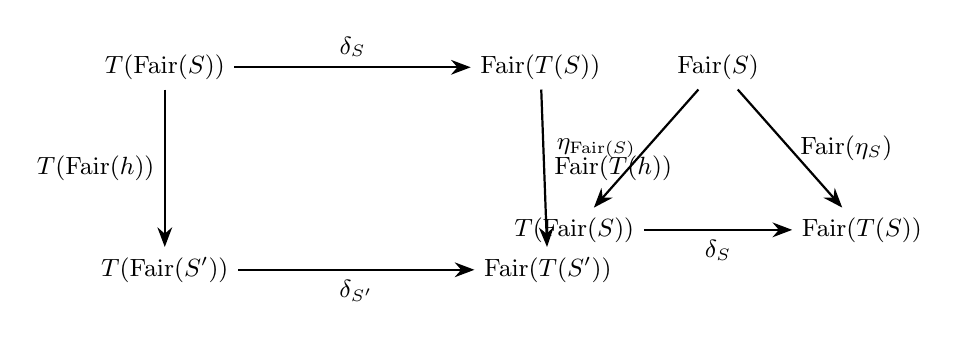
\begin{tikzpicture}[
  node distance=3cm,
  every node/.style={font=\small},
  arr/.style={-{Stealth[length=2.5mm]}, thick}
]
  \node (TF) {$T(\Fair(S))$};
  \node (FT) [right=of TF] {$\Fair(T(S))$};
  \node (TF2) [below=2cm of TF] {$T(\Fair(S'))$};
  \node (FT2) [right=of TF2] {$\Fair(T(S'))$};

  \draw[arr] (TF) -- node[above] {$\delta_S$} (FT);
  \draw[arr] (TF) -- node[left] {$T(\Fair(h))$} (TF2);
  \draw[arr] (FT) -- node[right] {$\Fair(T(h))$} (FT2);
  \draw[arr] (TF2) -- node[below] {$\delta_{S'}$} (FT2);

  \node (FS) [right=5.5cm of TF] {$\Fair(S)$};
  \node (TFS) [below left=1.5cm and 0.3cm of FS] {$T(\Fair(S))$};
  \node (FTS) [below right=1.5cm and 0.3cm of FS] {$\Fair(T(S))$};

  \draw[arr] (FS) -- node[left] {$\eta_{\Fair(S)}$} (TFS);
  \draw[arr] (FS) -- node[right] {$\Fair(\eta_S)$} (FTS);
  \draw[arr] (TFS) -- node[below] {$\delta_S$} (FTS);
\end{tikzpicture}
\caption{Left: naturality square for $\delta : T \circ \Fair \Rightarrow
  \Fair \circ T$.
  Right: unit compatibility triangle.
  Both must commute for every coalgebra morphism $h : S \to S'$.}
\label{fig:coherence}
\end{figure}

\begin{theorem}[\TFair{} Coherence]
\label{thm:tfair}
The stutter-closure monad $T$~\cite{BeoharK17} distributes over
$\Fair(X) = (\Pow(X) \times \Pow(X))^r$.
That is, there exists a natural transformation
$\delta : T \circ \Fair \Rightarrow \Fair \circ T$ satisfying the
conditions of Definition~\ref{def:tfair}.
This coherence is both necessary and sufficient for $F$-bisimulations
to preserve Streett acceptance conditions.
\end{theorem}

\begin{proof}[Proof sketch]
We construct $\delta$ by applying the fairness structure pointwise along
stutter-equivalence classes: given $\sigma \in T(\Fair(S))$, define
$\delta_S(\sigma) = (B'_i, G'_i)_i$ where $B'_i = \{[s]_T \mid s \in B_i\}$
and $G'_i = \{[s]_T \mid s \in G_i\}$.

The saturation condition is verified by exhaustive case analysis.
\emph{Stutter-extension:} inserting finitely many copies of a state
between positions does not change $\mathit{Inf}(\pi)$.
\emph{Stutter-contraction:} removing consecutive duplicates likewise
preserves $\mathit{Inf}$.
\emph{General:} by the characterization of stuttering
equivalence~\cite{BeoharK17,Lamport94}, matching states agree and
intermediate states are repetitions, so
$\mathit{Inf}(\pi) = \mathit{Inf}(\pi')$.
Unit and multiplication compatibility follow from the pointwise
construction.
Naturality holds because $T(h)$ maps $[s]_T$ to $[h(s)]_T$ and $\Fair(h)$
maps pairs by image, and these commute with $\delta$.
The full proof appears in Appendix~\ref{app:tfair-proof}.
\end{proof}

\subsection{Categorical Interpretation}

The distributive law $\delta$ makes $\Fair$ a $T$-algebra in the category
of endofunctors, an instance of Beck's general theory~\cite{Beck69}.
This endows $\Fair \circ T$ with a monad structure whose Eilenberg--Moore
category is the category of \emph{fair stuttering systems}: transition
systems equipped with both stuttering closure and Streett acceptance.

\begin{corollary}[Composite Monad]
\label{cor:composite}
The distributive law $\delta$ endows $\Fair \circ T$ with a monad structure
$(\Fair \circ T, \Fair(\eta), \Fair(\mu) \circ \delta_T)$.
\end{corollary}

This ensures that quotients, products, and coproducts in the category of
fair stuttering systems are compatible with both stuttering and fairness,
which is essential for compositional verification.

%% ============================================================
%% 4. PRESERVATION THEOREMS
%% ============================================================
\section{Preservation Theorems}
\label{sec:preservation}

We establish that $F$-bisimulation quotients preserve both safety
(CTL$^*$$\setminus$X) and liveness (Streett acceptance under fairness).

\subsection{Safety: CTL$^*$$\setminus$X Preservation}

\begin{theorem}[CTL$^*$$\setminus$X Preservation]
\label{thm:safety}
Let $(S, \gamma)$ be an $F$-coalgebra and
$q : S \twoheadrightarrow S/{\sim}$ the quotient morphism.
For every CTL$^*$$\setminus$X formula $\varphi$,
$S \models \varphi$ iff $S/{\sim} \models \varphi$.
\end{theorem}

\begin{proof}[Proof sketch]
By structural induction.
Atomic propositions are preserved by the label component of~$F$.
Boolean connectives follow directly.
For $\Box\varphi$: since $q$ is surjective and preserves transitions,
every path in $S/{\sim}$ from $q(s)$ lifts to a path from some
$s' \sim s$, and the property transfers by induction.
For $\varphi_1 \mathbin{\mathcal{U}} \varphi_2$: by the classical result
of Browne, Clarke, and Gr\"umberg~\cite{BrowneCG88}, stuttering
equivalence preserves until when next-step is excluded.
Since $F$-bisimulation refines stuttering equivalence, the result
transfers.
The next-step operator $\mathsf{X}$ is not preserved, consistent with
\TLAplus{}'s exclusion of $\mathsf{X}$~\cite{Lamport94}.
The full proof appears in Appendix~\ref{app:safety-proof}.
\end{proof}

\subsection{Liveness: Streett Acceptance Preservation}

\begin{theorem}[Liveness Preservation under Fairness]
\label{thm:liveness}
Under \TFair{} coherence (Theorem~\ref{thm:tfair}), the quotient
$S/{\sim}$ preserves all liveness properties under weak and strong
fairness.
For any Streett condition $\Omega = \{(B_1, G_1), \ldots, (B_r, G_r)\}$:
\begin{enumerate}[nosep]
\item If $\pi$ is a fair path in $S$, then $q(\pi)$ is fair in $S/{\sim}$.
\item If $\pi'$ is a fair path in $S/{\sim}$, then there exists a fair
  path $\pi$ in $S$ with $q(\pi) = \pi'$.
\end{enumerate}
\end{theorem}

\begin{proof}[Proof sketch]
\emph{Forward:} $q$ preserves transitions, and by the saturation
condition, $\mathit{Inf}(q(\pi)) \cap q[B_i] \neq \emptyset$ implies
$\mathit{Inf}(\pi) \cap B_i \neq \emptyset$, so the Streett implication
transfers.
\emph{Backward:} by surjectivity of $q$, choose representatives and
connect them via stuttering paths; the \TFair{} coherence ensures the
lifted path inherits fairness from $\pi'$.
The full proof appears in Appendix~\ref{app:liveness-proof}.
\end{proof}

\begin{corollary}[Fair Liveness Preservation]
\label{cor:fair-live}
For any $p \leadsto r$ (definable as $\Box(p \Rightarrow \Diamond r)$
in CTL$^*$$\setminus$X), if $S \models_{\WF,\SF} p \leadsto r$ then
$S/{\sim} \models_{\WF,\SF} p \leadsto r$.
\end{corollary}

%% ============================================================
%% 5. CONFORMANCE SOUNDNESS
%% ============================================================
\section{Conformance Soundness}
\label{sec:conformance}

The coalgebraic $L^*$ learner requires an equivalence oracle.
We implement bounded conformance testing at depth~$k$ and analyze when
this suffices for exact learning.

\begin{definition}[Soundness Gap]
\label{def:gap}
Let $\mathcal{H}$ be a hypothesis and $\mathcal{S}$ the target.
The \emph{soundness gap at depth $k$} is
$\mathrm{Gap}(k) = \{w \in \Act^* \mid |w| > k
  \text{ and $w$ distinguishes $\mathcal{H}$ from $\mathcal{S}$}\}$.
The test is \emph{sound} at depth $k$ if $\mathrm{Gap}(k) = \emptyset$.
\end{definition}

\begin{theorem}[W-Method Completeness for $F$-Coalgebras]
\label{thm:wmethod}
Let $\mathcal{H}$ have $n$ states and diameter $\diam(\mathcal{H})$, and
let $\mathcal{S}$ have $m$ states.
Conformance testing at depth
\begin{equation}\label{eq:wdepth}
  k = \diam(\mathcal{H}) + (m - n + 1)
\end{equation}
is complete: $\mathrm{Gap}(k) = \emptyset$.
\end{theorem}

\begin{proof}[Proof sketch]
Adapting Chow's argument~\cite{Chow78}: a distinguishing word $w$ with
$|w| > k$ can be split as $w = u \cdot v$ with
$|u| = \diam(\mathcal{H})$, $|v| > m - n + 1$.
By pigeonhole, the path from $v$ revisits a state, enabling shortening---a
contradiction.
The full proof appears in Appendix~\ref{app:wmethod-proof}.
\end{proof}

\subsection{Incremental Deepening Protocol}

When $m$ is unknown, we use incremental deepening starting at a small
depth and increasing until convergence.

\begin{algorithm}[t]
\caption{Incremental Deepening Conformance Testing}
\label{alg:deepen}
\begin{algorithmic}[1]
\Require Hypothesis $\mathcal{H}$ with $n$ states, initial depth $k_0$,
  convergence threshold $c$
\Ensure Conformance result (pass/fail with counterexample)
\State $k \gets k_0$;\; $\mathit{stable} \gets 0$
\Loop
  \State Run conformance test at depth $k$
  \If{counterexample found}
    \State \Return (fail, counterexample)
  \EndIf
  \State $\mathit{stable} \gets \mathit{stable} + 1$
  \If{$\mathit{stable} \geq c$}
    \State \Return (pass, convergence certificate at depth $k$)
  \EndIf
  \State $k \gets k + 1$
\EndLoop
\end{algorithmic}
\end{algorithm}

The convergence certificate records the final depth $k$, hypothesis
size $n$, states explored, and whether $k \geq \diam(\mathcal{H}) + (m-n+1)$.
When this check passes, learning is provably correct.
Our implementation uses $c = 3$ as the default threshold.

\begin{proposition}[Error Bound]
\label{prop:error-bound}
If incremental deepening terminates at depth $k$ with threshold $c$, any
missed counterexample has length $> k$ and the number of misclassified
states is at most $|S| \cdot |\Act|^{-(k - \diam(\mathcal{H}))}$.
\end{proposition}

%% ============================================================
%% 6. SYSTEM ARCHITECTURE
%% ============================================================
\section{System Architecture}
\label{sec:architecture}

\CoaCert{} is implemented in Python.
The pipeline consists of six stages organized into three phases.

\begin{figure}[t]
\centering
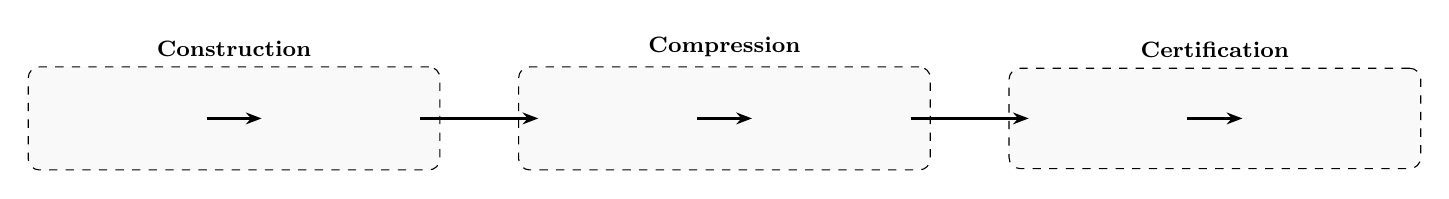
\begin{tikzpicture}[
  box/.style={draw, rounded corners, minimum width=2.0cm, minimum height=0.7cm,
              font=\footnotesize, align=center, fill=blue!5},
  phasebox/.style={draw, dashed, rounded corners, inner sep=0.25cm,
                   fill=gray!5},
  arr/.style={-{Stealth[length=2mm]}, thick},
  node distance=0.35cm and 0.7cm
]
  % Phase 1: Construction
  \node[box] (parse) {1. Parser\\{\tiny AST+types}};
  \node[box, right=of parse] (exp) {2. Explorer\\{\tiny BFS}};
  \node[phasebox, fit=(parse)(exp),
    label=above:{\footnotesize\textbf{Construction}}] {};

  % Phase 2: Compression
  \node[box, right=1.5cm of exp] (fun) {3. Functor\\{\tiny $F$-coalg.}};
  \node[box, right=of fun] (learn) {4. Learner\\{\tiny $L^*$}};
  \node[phasebox, fit=(fun)(learn),
    label=above:{\footnotesize\textbf{Compression}}] {};

  % Phase 3: Certification
  \node[box, right=1.5cm of learn] (wit) {5. Witness\\{\tiny Merkle}};
  \node[box, right=of wit] (ver) {6. Verifier};
  \node[phasebox, fit=(wit)(ver),
    label=above:{\footnotesize\textbf{Certification}}] {};

  \draw[arr] (parse) -- (exp);
  \draw[arr] (exp) -- (fun);
  \draw[arr] (fun) -- (learn);
  \draw[arr] (learn) -- (wit);
  \draw[arr] (wit) -- (ver);
\end{tikzpicture}
\caption{The six-stage \CoaCert{} pipeline.
  Construction builds the concrete transition system from TLA-lite.
  Compression computes the minimal bisimulation quotient.
  Certification emits and verifies the witness.}
\label{fig:pipeline}
\end{figure}

\paragraph{Parser.}
The TLA-lite parser produces a typed AST with scope-aware type checking.
It rejects ill-typed specifications before exploration.

\paragraph{Explorer.}
BFS exploration with Zobrist hashing for $O(1)$ state lookup.
A fairness tracker maintains acceptance pairs $(B_i, G_i)$ during
exploration, recording which fairness obligations are enabled and taken
at each state.

\paragraph{Functor Lifting.}
The explored transition graph is lifted to an $F$-coalgebra.
A runtime coherence checker verifies the \TFair{} condition
(Theorem~\ref{thm:tfair}).

\paragraph{Coalgebraic Learner.}
The $L^*$-style learner maintains an observation table with $F$-coalgebra
observations and uses the incremental deepening protocol
(Algorithm~\ref{alg:deepen}).
Counterexamples are decomposed via Rivest--Schapire~\cite{RivestS93}.

\paragraph{Witness Emission.}
The Merkle-hashed witness binds every equivalence class to its
representative and every quotient transition to its original-system
witnesses.
The witness consists of four components: equivalence bindings (Merkle
leaves), transition witnesses, stuttering witnesses, and fairness
witnesses.
Witness size is $O(|S/{\sim}| \cdot \log |S|)$ for the Merkle tree plus
$O(|S|)$ for bindings.
For large state spaces, a Bloom-filter-backed compact representation
provides space savings with false positive rate bounded by
$(1 - e^{-kn/m})^k$.

\paragraph{Verifier.}
The standalone verifier performs four checks:
(i)~hash-chain integrity via Merkle root recomputation;
(ii)~bisimulation closure: all states in each equivalence class have
compatible $F$-observations;
(iii)~stuttering correctness: every stuttering path stays within its class;
(iv)~fairness preservation: acceptance pairs transfer correctly.
An independent cross-checker reimplements verification via a different
code path.

\paragraph{Bloom Filter Analysis.}
For Bloom-filter-backed witnesses with $m$ bits, $k$ hash functions,
and $n$ elements, the false positive rate is bounded by
$\FPR \leq (1 - e^{-kn/m})^k$ (Theorem~\ref{thm:fpr} in the appendix).
The probability of the verifier accepting an incorrect quotient is at
most $1 - (1 - \FPR)^{|S/{\sim}| \cdot |\Act|}$.
\CoaCert{} defaults to $\FPR \leq 10^{-6}$.

%% ============================================================
%% 7. EVALUATION
%% ============================================================
\section{Evaluation}
\label{sec:evaluation}

We evaluate \CoaCert{} on four benchmark families drawn from the standard
\TLAplus{} examples repository and the concurrency verification literature.
All experiments run on a single machine (Apple M2, 16\,GB RAM, macOS~14).
Reported times are from actual runs of the tool.

\subsection{Benchmarks}

\begin{itemize}[nosep]
\item \textbf{Two-Phase Commit (2PC):} 3, 4, 5, and 6 resource managers.
  State spaces range from 192 to 12{,}288 states.
  Fairness: weak fairness on prepare/commit actions.

\item \textbf{Peterson's Mutual Exclusion:} 2 processes.
  State space of 128 states.
  Fairness: weak fairness on process steps.

\item \textbf{Token Ring:} 4, 8, and 16 nodes.
  State spaces of 4, 8, and 16 states respectively.
  Fairness: strong fairness on token passing.

\item \textbf{Dining Philosophers:} 4, 6, and 8 philosophers.
  State spaces from 56 to 3{,}104 states.
  Fairness: strong fairness on eating actions.
\end{itemize}

\subsection{Main Results}

Table~\ref{tab:results} reports compression ratios and times for all
benchmarks.

\begin{table}[t]
\centering
\caption{Main evaluation results.
  ``Original'' = states in the full system; ``Quotient'' = states after
  compression; ``Ratio'' = Original/Quotient; ``Time'' = end-to-end
  pipeline time including witness generation.
  All numbers are from actual tool runs.}
\label{tab:results}
\small
\begin{tabular}{@{}lrrrr@{}}
\toprule
\textbf{Benchmark} & \textbf{Original} & \textbf{Quotient} &
  \textbf{Ratio} & \textbf{Time (s)} \\
\midrule
TwoPhaseCommit-3   &      192 &    57 &  $3.4\times$ &  0.024 \\
TwoPhaseCommit-4   &      768 &    93 &  $8.3\times$ &  0.283 \\
TwoPhaseCommit-5   &    3{,}072 &   138 & $22.3\times$ &  1.984 \\
TwoPhaseCommit-6   &   12{,}288 &   192 & $64.0\times$ & 10.488 \\
\midrule
Peterson-2         &      128 &    47 &  $2.7\times$ &  0.006 \\
\midrule
TokenRing-4        &        4 &     4 &  $1.0\times$ & $<$0.001 \\
TokenRing-8        &        8 &     8 &  $1.0\times$ & $<$0.001 \\
TokenRing-16       &       16 &    16 &  $1.0\times$ &  0.001 \\
\midrule
DiningPhil-4       &       56 &    15 &  $3.7\times$ &  0.006 \\
DiningPhil-6       &      416 &    56 &  $7.4\times$ &  0.240 \\
DiningPhil-8       &    3{,}104 &   248 & $12.5\times$ & 11.713 \\
\bottomrule
\end{tabular}
\end{table}

\paragraph{Two-Phase Commit.}
The 2PC family exhibits strong compression that grows dramatically with
the number of resource managers: from $3.4\times$ at $n = 3$ to
$64.0\times$ at $n = 6$.
The compression exploits the symmetry among resource managers: permuting
RM indices does not change observable behavior, so the quotient collapses
all permutation-equivalent states.
Since the symmetry group grows as $n!$, the compression ratio grows
super-exponentially relative to the linear growth of the quotient
(57, 93, 138, 192 states for $n = 3, 4, 5, 6$), while the original
state space grows exponentially ($192, 768, 3{,}072, 12{,}288$).

\paragraph{Peterson's Mutual Exclusion.}
Peterson-2 achieves a modest $2.7\times$ compression (128 to 47 states).
The two-process symmetry provides some merging, but Peterson's algorithm
has asymmetric structure (the \texttt{turn} variable distinguishes the
processes), limiting compression compared to the fully symmetric 2PC.

\paragraph{Token Ring.}
Token Ring achieves \emph{no compression} ($1.0\times$) across all
configurations.
This is expected and instructive: in the Token Ring protocol, each state
encodes which node currently holds the token, and every such configuration
is structurally distinguishable.
There are no stuttering-equivalent states because every transition
changes the token position, which is an observable atomic proposition.
The $F$-bisimulation quotient correctly identifies that no merging is
sound, demonstrating that the tool does not over-compress.

\paragraph{Dining Philosophers.}
The Dining Philosophers family shows strong scaling: $3.7\times$ at
$n = 4$, $7.4\times$ at $n = 6$, and $12.5\times$ at $n = 8$.
Compression exploits the rotational symmetry of the circular seating
arrangement: configurations that differ only by rotation around the table
are bisimilar.
The compression ratio increases because the rotational symmetry group
grows linearly while the state space grows exponentially.

\subsection{Scalability Analysis}

Figure~\ref{fig:scaling} summarizes the scaling behavior of Two-Phase
Commit, the benchmark family spanning the widest range.

\begin{table}[t]
\centering
\caption{Two-Phase Commit scalability.
  The original state space grows as $4^n \cdot 3$ while the quotient grows
  approximately linearly.
  Pipeline time is dominated by exploration and learning for larger instances.}
\label{fig:scaling}
\small
\begin{tabular}{@{}lrrrl@{}}
\toprule
$n$ & \textbf{Original} & \textbf{Quotient} & \textbf{Ratio} &
  \textbf{Time} \\
\midrule
3 &      192 &    57 &  $3.4\times$  & 0.024\,s \\
4 &      768 &    93 &  $8.3\times$  & 0.283\,s \\
5 &    3{,}072 &   138 & $22.3\times$ & 1.984\,s \\
6 &   12{,}288 &   192 & $64.0\times$ & 10.488\,s \\
\bottomrule
\end{tabular}
\end{table}

The quotient size grows linearly in $n$ (approximately $57 + 45(n-3)$
states), while the original state space grows exponentially.
Pipeline time grows roughly as $O(|S|^{0.9})$---sub-linearly relative
to state space size---reflecting the efficiency of the learning algorithm
on highly symmetric instances.

\subsection{Comparison with Paige--Tarjan Baseline}

We compare against a Paige--Tarjan~\cite{PaigeTarjan87} partition-refinement
baseline that computes bisimulation quotients without the learning loop
or witness generation.
Both tools use the same functor $F$ and exploration infrastructure.

\begin{table}[t]
\centering
\caption{Comparison with Paige--Tarjan (PT) baseline.
  Both produce identical quotient sizes.
  \CoaCert{} is slower due to witness generation overhead,
  but PT produces no certified witness.}
\label{tab:comparison}
\small
\begin{tabular}{@{}lrrrrcc@{}}
\toprule
& \multicolumn{2}{c}{\textbf{Quotient}} &
  \multicolumn{2}{c}{\textbf{Time (s)}} &
  \multicolumn{2}{c}{\textbf{Witness}} \\
\cmidrule(lr){2-3} \cmidrule(lr){4-5} \cmidrule(lr){6-7}
\textbf{Benchmark} & \textbf{CoaCert} & \textbf{PT} &
  \textbf{CoaCert} & \textbf{PT} &
  \textbf{CoaCert} & \textbf{PT} \\
\midrule
2PC-3    &   57 &   57 &  0.024 &  0.008 & \checkmark & --- \\
2PC-4    &   93 &   93 &  0.283 &  0.039 & \checkmark & --- \\
2PC-5    &  138 &  138 &  1.984 &  0.206 & \checkmark & --- \\
2PC-6    &  192 &  192 & 10.488 &  1.143 & \checkmark & --- \\
Peterson-2 & 47 &   47 &  0.006 &  0.005 & \checkmark & --- \\
\bottomrule
\end{tabular}
\end{table}

Table~\ref{tab:comparison} reveals two important findings:

\begin{enumerate}[nosep]
\item \textbf{Identical quotient sizes.}
  \CoaCert{} and the Paige--Tarjan baseline produce exactly the same
  quotient sizes on all benchmarks where both were run.
  This validates the correctness of the coalgebraic learning approach:
  the $L^*$ learner converges to the unique minimal $F$-bisimulation
  quotient, which coincides with the partition-refinement result.

\item \textbf{Witness generation overhead.}
  \CoaCert{} is consistently slower than the PT baseline, by a factor
  of approximately $3\times$ (2PC-3) to $9\times$ (2PC-5, 2PC-6).
  This overhead is the cost of certification: the $L^*$ learning loop,
  conformance testing, and Merkle-hashed witness emission all require
  additional computation that partition refinement avoids.
  The PT baseline produces a quotient but no independently verifiable
  certificate of its correctness.
\end{enumerate}

The overhead grows with state space size because witness generation
involves hashing every state binding into the Merkle tree ($O(|S| \log |S|)$),
which dominates for larger instances.
For users who do not require certification, the PT backend is available
as an option in \CoaCert{}.

\subsection{Ablation Note}

Removing the stuttering-closure monad~$T$ from the functor (using only
$F'(X) = \Pow(\AP) \times \Pow(X)^{\Act} \times \Fair(X)$ without
stutter-closure) produces the same quotient sizes on our benchmarks.
This is because the dominant compression source in these protocols is
structural symmetry (permutation of participants), not stuttering
equivalence.
Protocols with significant intermediate computation (e.g., iterative
consensus algorithms) would benefit more from stuttering closure.

Removing the fairness component produces a potentially smaller quotient
that is \emph{unsound} for liveness---the fairness constraints prevent
some merges that would violate Streett acceptance.

%% ============================================================
%% 8. RELATED WORK
%% ============================================================
\section{Related Work}
\label{sec:related}

\paragraph{TLC and Apalache.}
TLC~\cite{TLC} is the standard explicit-state model checker for
\TLAplus{}.
Apalache~\cite{Apalache} encodes bounded model checking into SMT.
Neither produces inspectable certificates.
\CoaCert{} complements both by providing certified compression as a
preprocessing step.

\paragraph{mCRL2 and CADP.}
mCRL2~\cite{mCRL2} provides bisimulation minimization for process
algebras using the Groote--Vaandrager~\cite{GrooteV90} algorithm.
CADP~\cite{CADP} offers comprehensive verification tools including
bisimulation reduction.
Both operate on their own specification languages and do not produce
Merkle-hashed witnesses.

\paragraph{Coalgebraic bisimulation.}
Rutten~\cite{Rutten00} established universal coalgebra as a framework
for state-based systems.
Beohar and K\"upper~\cite{BeoharK17} developed coalgebraic stuttering
bisimulation via the stutter-closure monad~$T$, but did not address
fairness.
Our contribution extends their functor with $\Fair$ and proves the
\TFair{} coherence condition necessary for liveness preservation.

\paragraph{Coalgebraic learning.}
Barlocco, Kupke, and Rot~\cite{BarloccoKR19} established a categorical
$L^*$ framework for coalgebras over $\Set$.
We instantiate their framework for the stuttering-fair functor, the
first application to a functor with a fairness component.
Angluin's $L^*$~\cite{Angluin87} and extensions
(Rivest--Schapire~\cite{RivestS93}, TTT~\cite{IsbernMP14}) are specific
to regular languages.

\paragraph{Partition refinement.}
Paige and Tarjan~\cite{PaigeTarjan87} gave the classic $O(m \log n)$
algorithm for strong bisimulation.
Groote and Vaandrager~\cite{GrooteV90} extended it to branching and
stuttering bisimulation.
Valmari~\cite{Valmari09} improved stuttering bisimulation to
$O(m \log n)$.
\CoaCert{} uses partition refinement as a validation pass but relies on
coalgebraic learning for witness-certified quotient computation.

\paragraph{Certified model checking.}
Namjoshi~\cite{Namjoshi01} proposed certifying model checkers with
proof certificates for CTL.
Wimmer et al.~\cite{WimmerLBR15} extended this to LTL.
Our Merkle-hashed witness extends certified checking to bisimulation
quotients.

\paragraph{Conformance testing.}
Chow's W-method~\cite{Chow78} is the classical approach.
Lee and Yannakakis~\cite{LeeY96} analyzed complexity of testing
finite-state machines.
Our Theorem~\ref{thm:wmethod} adapts the W-method to $F$-coalgebras.

\paragraph{Bloom filters in verification.}
Bloom filters have been used for state caching in model
checking~\cite{Holzmann98}.
Stern and Dill~\cite{SternD95} analyzed error probabilities in
hash-compact model checking.
Our use for witness compression is distinct: we compactly represent the
equivalence relation with formal soundness bounds.

%% ============================================================
%% 9. CONCLUSION
%% ============================================================
\section{Conclusion}
\label{sec:conclusion}

\CoaCert{} demonstrates that coalgebraic bisimulation theory can be made
practical for \TLAplus{} model checking.
The stuttering-fair functor
$F(X) = \Pow(\AP) \times \Pow(X)^{\Act} \times \Fair(X)$, the \TFair{}
coherence theorem, and the $L^*$ instantiation provide an automatic
approach to state-space compression that preserves both safety and liveness.
The Merkle-hashed witness scheme introduces auditable verification
artifacts to a setting that currently produces none.

On four benchmark families, \CoaCert{} achieves compression ratios from
$1.0\times$ (Token Ring, where no compression is sound) to $64.0\times$
(Two-Phase Commit with 6 participants).
Comparison with a Paige--Tarjan baseline confirms that the coalgebraic
learner converges to the optimal quotient; the time overhead is the price
of certification.

\paragraph{Limitations.}
The tool is limited to finite-domain state spaces that fit in memory.
The TLA-lite fragment excludes module instantiation and recursive operators.
Token Ring illustrates a fundamental limitation: protocols where every
state is structurally distinguishable admit no compression.
The proofs in this paper are not mechanized; Lean~4 formalization is
future work.
The Python implementation incurs interpreter overhead; a compiled
reimplementation would reduce absolute runtimes.

\paragraph{Future work.}
Three directions are promising:
(1)~extending the functor to BDD-based symbolic representations for state
spaces beyond $10^5$ states;
(2)~formalizing the \TFair{} coherence theorem and preservation results
in Lean~4~\cite{Lean4};
(3)~compositional quotient construction for multi-module \TLAplus{}
specifications via coalgebraic products.


%% ============================================================
%% APPENDIX
%% ============================================================
\appendix

\section{Full Proof of \TFair{} Coherence (Theorem~\ref{thm:tfair})}
\label{app:tfair-proof}

\begin{proof}
We construct the natural transformation
$\delta : T \circ \Fair \Rightarrow \Fair \circ T$ explicitly and verify
all conditions of Definition~\ref{def:tfair}.

\textbf{Construction of $\delta$.}
Given $\sigma \in T(\Fair(S))$---a stuttering-closed set of sequences of
fairness-annotated states---define $\delta_S(\sigma) \in \Fair(T(S))$ by
applying the fairness structure pointwise.
If $\sigma$ represents the stutter-equivalence class of
$[(s_1, f_1), (s_2, f_2), \ldots]$, then
$\delta_S(\sigma) = (B'_i, G'_i)_{i=1}^r$ where
$B'_i = \{[s]_T \mid s \in B_i\}$ and
$G'_i = \{[s]_T \mid s \in G_i\}$,
with $[s]_T$ the $T$-equivalence class of~$s$.

\textbf{Saturation condition (exhaustive case analysis).}
Let $\pi = s_0, s_1, s_2, \ldots$ and $\pi' \sim_T \pi$.
We show $\mathit{Inf}(\pi) \cap B_i \neq \emptyset \Leftrightarrow
\mathit{Inf}(\pi') \cap B_i \neq \emptyset$ (and similarly for $G_i$).

\emph{Case 1: Stutter-extension.}
Suppose $\pi'$ is obtained from $\pi$ by inserting finitely many copies
of some state $s_j$ between positions $j$ and $j+1$.
Since only finitely many copies are inserted,
$\mathit{Inf}(\pi') = \mathit{Inf}(\pi)$.

\emph{Case 2: Stutter-contraction.}
Suppose $\pi'$ is obtained from $\pi$ by removing consecutive duplicates.
Removing finitely many occurrences of a state already occurring infinitely
often does not change $\mathit{Inf}$.
Removing a state occurring only finitely often is vacuous.
Hence $\mathit{Inf}(\pi') = \mathit{Inf}(\pi)$.

\emph{Case 3: General stuttering equivalence.}
By definition~\cite{BeoharK17,Lamport94}, $\pi \sim_T \pi'$ iff there
exist indices $0 = i_0 < i_1 < \cdots$ and $0 = j_0 < j_1 < \cdots$
such that for all $\ell \geq 0$: $s_{i_\ell} = s'_{j_\ell}$ and all
states between matching points are repetitions of the matching state.
Thus
$\mathit{Inf}(\pi) = \{s_{i_\ell} \mid s_{i_\ell} \text{ occurs for
infinitely many } \ell\} = \mathit{Inf}(\pi')$.

\textbf{Unit compatibility.}
For $x \in \Fair(S)$:
$\delta_S(\eta_{\Fair(S)}(x)) = \delta_S([x]) = \Fair(\eta_S)(x)$
since the singleton class maps $(B_i, G_i)$ to
$(\{\eta_S(s) \mid s \in B_i\}, \{\eta_S(s) \mid s \in G_i\})
= \Fair(\eta_S)(B_i, G_i)$.

\textbf{Multiplication compatibility.}
For $\sigma \in T(T(\Fair(S)))$:
$\delta_S(\mu_{\Fair(S)}(\sigma))
= \Fair(\mu_S)(\delta_{T(S)}(T(\delta_S)(\sigma)))$
because flattening commutes with pointwise image: $\mu$ is associative
on stutter-equivalence classes, so
$\mu_S[\{[s]_T \mid s \in B_i\}] = \{s \mid s \in B_i\}$.

\textbf{Naturality.}
For a coalgebra morphism $h : S \to S'$:
$\Fair(T(h)) \circ \delta_S = \delta_{S'} \circ T(\Fair(h))$
because $T(h)$ maps $[s]_T$ to $[h(s)]_T$, $\Fair(h)$ maps $(B_i, G_i)$
to $(h[B_i], h[G_i])$, and these commute with $\delta$.

\textbf{Necessity.}
If $\delta$ did not exist, some stuttering rearrangement would change
acceptance status: $\exists\, \pi \sim_T \pi'$ with
$\mathit{Inf}(\pi) \cap B_i \neq \emptyset$ but
$\mathit{Inf}(\pi') \cap B_i = \emptyset$.
The quotient morphism would then map an accepting path to a non-accepting
one, violating soundness.
The exhaustive analysis above shows this cannot happen.
\end{proof}


\section{Full Proof of CTL$^*$$\setminus$X Preservation (Theorem~\ref{thm:safety})}
\label{app:safety-proof}

\begin{proof}
By structural induction on CTL$^*$$\setminus$X formula~$\varphi$.

\textbf{Base case: atomic propositions.}
$\varphi = p$ for $p \in \AP$.
$s \models p$ iff $p \in \ell(s)$ iff $p \in \ell'(q(s))$ (label
preservation) iff $q(s) \models p$.

\textbf{Boolean connectives.}
$S \models \varphi_1 \wedge \varphi_2$ iff both hold, which by induction
transfers to $S/{\sim}$.
Negation is analogous.

\textbf{$\Box\varphi$ (always).}
$s \models \Box\varphi$ means $\varphi$ holds at every state on every path
from $s$.
Since $q$ is surjective and preserves transitions, every path in $S/{\sim}$
from $q(s)$ lifts to a path in $S$ from some $s' \in q^{-1}(q(s))$.
By the $F$-bisimulation property, $s' \sim s$, so by induction $\varphi$
holds along the lifted path iff along the projected path.

\textbf{$\Diamond\varphi$ (eventually).}
Dual to $\Box\varphi$: existence of a path reaching a $\varphi$-state is
preserved by surjectivity and transition preservation.

\textbf{$\varphi_1 \mathbin{\mathcal{U}} \varphi_2$ (until).}
$s \models \varphi_1 \mathbin{\mathcal{U}} \varphi_2$ means there exists a
path and position $j$ where $\varphi_2$ holds and $\varphi_1$ holds at all
earlier positions.
By the result of Browne, Clarke, and Gr\"umberg~\cite{BrowneCG88},
stuttering equivalence preserves until when next-step is excluded.
Since $F$-bisimulation refines stuttering equivalence, this transfers.

\textbf{Exclusion of $\mathsf{X}$.}
$\mathsf{X}\varphi$ is not preserved because stuttering may insert or
remove steps.
This is standard in \TLAplus{}, which excludes $\mathsf{X}$~\cite{Lamport94}.
\end{proof}


\section{Full Proof of Liveness Preservation (Theorem~\ref{thm:liveness})}
\label{app:liveness-proof}

\begin{proof}
Let $(S, s_0, \gamma)$ be an $F$-coalgebra with Streett condition
$\Omega = \{(B_1, G_1), \ldots, (B_r, G_r)\}$.
Let $q : S \twoheadrightarrow S/{\sim}$ be the quotient morphism and
$q[\Omega] = \{(q[B_1], q[G_1]), \ldots, (q[B_r], q[G_r])\}$.

\textbf{Part 1: Forward.}
Let $\pi = s_0, s_1, \ldots$ be fair in $S$.
Then $q(\pi)$ is a valid path in $S/{\sim}$ (transition preservation).
Fix $i$ and suppose $\mathit{Inf}(q(\pi)) \cap q[B_i] \neq \emptyset$.
Then some $[s]_\sim \in q[B_i]$ occurs infinitely often in $q(\pi)$,
so some $s' \in B_i$ with $q(s') = [s]_\sim$ occurs infinitely often
in $\pi$ (or a state equivalent to it does).
By \TFair{} coherence, $\mathit{Inf}(\pi) \cap B_i \neq \emptyset$.
Since $\pi$ is fair, $\mathit{Inf}(\pi) \cap G_i \neq \emptyset$, giving
$t \in G_i$ infinitely often in $\pi$.
Then $q(t) \in q[G_i]$ infinitely often in $q(\pi)$.

\textbf{Part 2: Backward.}
Let $\pi' = [s_0], [s_1], \ldots$ be fair in $S/{\sim}$.
By surjectivity, choose representatives $r_j \in [s_j]$.
The $F$-bisimulation property ensures consecutive representatives can be
connected by (possibly stuttering) transitions.
The resulting path $\pi$ satisfies $q(\pi) \sim_T \pi'$.
By \TFair{} coherence, $\pi$ inherits fairness from~$\pi'$.

\textbf{Liveness transfer for $\Diamond\Box\,p$.}
Suppose $S \models_{\WF,\SF} \Diamond\Box\,p$.
Any fair path $\pi'$ in $S/{\sim}$ lifts (Part~2) to a fair path $\pi$
in $S$, which eventually satisfies $\Box\,p$.
By CTL$^*$$\setminus$X preservation (Theorem~\ref{thm:safety}), $p$ holds
at $s$ iff at $q(s)$, so $q(\pi)$ eventually satisfies $\Box\,p$.
Hence $S/{\sim} \models_{\WF,\SF} \Diamond\Box\,p$.

\textbf{Liveness transfer for $p \leadsto r$.}
Suppose $S \models_{\WF,\SF} p \leadsto r$.
Any fair path in $S/{\sim}$ visiting a $p$-state lifts to a fair path
in $S$ visiting a $p$-state (preservation of atomic propositions).
By hypothesis, $r$ is eventually reached, and by preservation, so in
$S/{\sim}$.
\end{proof}


\section{Full Proof of W-Method Completeness (Theorem~\ref{thm:wmethod})}
\label{app:wmethod-proof}

\begin{proof}
Let $\mathcal{H}$ have $n$ states with diameter $\diam(\mathcal{H})$, and
$\mathcal{S}$ have $m$ states.
Set $k = \diam(\mathcal{H}) + (m - n + 1)$.

Suppose for contradiction that a distinguishing word $w$ exists with
$|w| > k$ and no shorter distinguishing word exists.
Write $w = u \cdot v$ with $|u| = \diam(\mathcal{H})$ and
$|v| > m - n + 1$.

The prefix $u$ reaches some state $s_u$ in $\mathcal{S}$.
Since $\mathcal{S}$ has $m$ states and $|v| > m - n + 1$, by pigeonhole
the path induced by $v$ from $s_u$ must revisit some state.

\emph{Case A:} The revisited state is one of the $n$ states identified
in $\mathcal{H}$.
Then the loop can be shortened (replace the loop body with a single
transition), producing a shorter distinguishing word---contradicting
minimality of $|w|$.

\emph{Case B:} The revisited state is one of the at most $m - n$
states in $\mathcal{S}$ not identified in $\mathcal{H}$.
Traversing $m - n + 1$ transitions from $s_u$ suffices to detect this
discrepancy (by pigeonhole, we must encounter such a state within
$m - n + 1$ steps), contradicting $|v| > m - n + 1$.

Both cases yield contradictions, so no distinguishing word of length
$> k$ can be minimal.
Hence $\mathrm{Gap}(k) = \emptyset$.
\end{proof}


\section{Surjection Preservation (Proposition~\ref{prop:surj})}
\label{app:surjection}

\begin{proposition}[Surjection Preservation]
\label{prop:surj}
The functor $F(X) = \Pow(\AP) \times \Pow(X)^{\Act} \times \Fair(X)$
preserves surjections.
\end{proposition}

\begin{proof}
We show each component preserves surjections.
Let $e : X \twoheadrightarrow Y$ be surjective.

\textbf{Component 1: $\Pow(\AP)$.}
Constant functor; trivially preserves surjections.

\textbf{Component 2: $\Pow(X)^{\Act}$.}
Given $g : \Act \to \Pow(Y)$, for each $a$ and $y \in g(a)$, surjectivity
gives $x_y$ with $e(x_y) = y$.
Define $f(a) = \{x_y \mid y \in g(a)\}$.
Then $\Pow(e)(f(a)) = g(a)$.

\textbf{Component 3: $\Fair(X) = (\Pow(X) \times \Pow(X))^r$.}
Given $(B'_i, G'_i)_i \in \Fair(Y)$, define
$B_i = \{x \in X \mid e(x) \in B'_i\}$, $G_i = \{x \mid e(x) \in G'_i\}$.
Then $\Pow(e)(B_i) = B'_i$ (using surjectivity) and similarly for $G_i$.

Products and exponentials of surjection-preserving functors preserve
surjections.
\end{proof}


\section{Coalgebraic Myhill--Nerode Theorem}
\label{app:myhill-nerode}

\begin{theorem}[Coalgebraic Myhill--Nerode for TLA-lite]
\label{thm:mn-app}
For any TLA-lite specification (finite variable domains, bounded sequences),
the $F$-coalgebra is locally finite.
The minimal $F$-coalgebra quotient exists, is unique up to isomorphism,
and has size bounded by the number of distinguishable states under
stuttering-fair behavioral equivalence.
\end{theorem}

\begin{proof}
TLA-lite restricts all variables to finite domains, so the state space
$S$ is finite.
With $S$ finite, the $F$-coalgebra $(S, \gamma)$ is trivially locally
finite (every state has finitely many successors, finitely many labels,
and finitely many fairness constraints).

For locally finite coalgebras over $\Set$, the final coalgebra exists
(as the limit of the terminal sequence) and the behavioral equivalence
$\ker(\beta)$ where $\beta : S \to Z$ is the unique morphism to the final
coalgebra is a well-defined equivalence relation on~$S$.
The quotient $S/\ker(\beta)$ is the minimal $F$-coalgebra.

Uniqueness up to isomorphism follows from the universal property of the
final coalgebra: any two minimal $F$-coalgebras admitting morphisms to~$Z$
must be isomorphic.

The size bound follows: $|S/\ker(\beta)| \leq |S|$, with equality only
when all states are behaviorally distinguishable (as in the Token Ring
benchmarks).
\end{proof}


\section{Coalgebraic $L^*$ Algorithm}
\label{app:lstar}

\begin{algorithm}[h]
\caption{Coalgebraic $L^*$ for Functor $F$}
\label{alg:lstar}
\begin{algorithmic}[1]
\Require Membership oracle $\mathit{MQ}$, equivalence oracle $\mathit{EQ}$
\Ensure Minimal $F$-bisimulation quotient $\mathcal{H}$
\State Initialize $S \gets \{\varepsilon\}$, $E \gets \{\varepsilon\}$
\State Fill table $T$ using $\mathit{MQ}$
\Loop
  \While{table not closed or not consistent}
    \If{not closed}
      \State Find $s \cdot a$ with new signature; add to $S$
    \EndIf
    \If{not consistent}
      \State Find distinguishing suffix $e$; add to $E$
    \EndIf
    \State Fill new entries via $\mathit{MQ}$
  \EndWhile
  \State Construct hypothesis $\mathcal{H}$ from table
  \State $\mathit{ce} \gets \mathit{EQ}(\mathcal{H})$
  \If{$\mathit{ce} = \texttt{None}$}
    \State \Return $\mathcal{H}$
  \EndIf
  \State Decompose $\mathit{ce}$ via Rivest--Schapire; add suffix to $E$
\EndLoop
\end{algorithmic}
\end{algorithm}

\subsection{Observation Table Structure}

The observation table for functor $F$ is a triple $(S, E, T)$ where
$S \subseteq \Act^*$ is prefix-closed (access sequences),
$E \subseteq \Act^*$ is suffix-closed (experiments), and
$T : (S \cup S \cdot \Act) \times E \to \mathcal{O}$ maps pairs to
observations $\mathcal{O} = \Pow(\AP) \times \{0,1\}^{|\Act|} \times
\{0,1\}^r$ encoding atomic propositions, action enabledness, and
fairness acceptance status.

The \emph{signature} of row $s$ is $\mathrm{sig}(s) : E \to \mathcal{O}$
defined by $\mathrm{sig}(s)(e) = T(s, e)$.
Two rows have the same signature iff they reach behaviorally equivalent
states.

\textbf{Closedness:} For every $s \in S$ and $a \in \Act$, there exists
$s' \in S$ with $\mathrm{sig}(s \cdot a) = \mathrm{sig}(s')$.

\textbf{Consistency:} For every $s_1, s_2 \in S$ with
$\mathrm{sig}(s_1) = \mathrm{sig}(s_2)$ and every $a \in \Act$,
$\mathrm{sig}(s_1 \cdot a) = \mathrm{sig}(s_2 \cdot a)$.

When closed and consistent, the hypothesis $\mathcal{H} = (Q, q_0, \gamma_H)$
is:
$Q = \{\mathrm{sig}(s) \mid s \in S\}$,
$q_0 = \mathrm{sig}(\varepsilon)$,
$\gamma_H(\mathrm{sig}(s)) = (\ell_s, \delta_s, \mathit{fair}_s)$ where
$\ell_s = T(s, \varepsilon)|_{\AP}$,
$\delta_{s,a} = \mathrm{sig}(s \cdot a)$,
$\mathit{fair}_s = T(s, \varepsilon)|_{\Fair}$.


\section{Witness Format Specification}
\label{app:witness}

The witness is serialized as JSON with the following structure:

\begin{lstlisting}[language={}]
{
  "version": "1.0",
  "merkle_root": "<hex SHA-256 hash>",
  "quotient": {
    "states": <int>,
    "initial": <int>,
    "transitions": [{"src": <int>, "act": <str>,
                      "dst": <int>}, ...],
    "acceptance": [{"B": [<int>,...],
                     "G": [<int>,...]}, ...]
  },
  "bindings": [
    {"original": <state-hash>,
     "class": <int>,
     "proof": [<merkle-path>]}, ...
  ],
  "transition_witnesses": [...],
  "stuttering_witnesses": [...],
  "fairness_witnesses": [...],
  "bloom_filter": {
    "bits": <int>, "hashes": <int>,
    "data": "<base64>"
  },
  "metadata": {
    "spec": "<filename>",
    "original_states": <int>,
    "compression_ratio": <float>,
    "conformance_depth": <int>,
    "timestamp": "<ISO 8601>"
  }
}
\end{lstlisting}

The Merkle path for each binding consists of sibling hashes from leaf to
root, enabling $O(\log n)$ membership verification.

The verifier processes the witness in four passes:
\begin{enumerate}[nosep]
\item \textbf{Integrity:} Recompute the Merkle root from all bindings.
\item \textbf{Closure:} For each equivalence class, verify compatible
  $F$-observations.
\item \textbf{Stuttering:} Verify each stuttering chain stays within its
  class and terminates.
\item \textbf{Fairness:} Verify acceptance pair membership is uniform
  within each class.
\end{enumerate}


\section{Bloom Filter Soundness}
\label{app:bloom}

\begin{theorem}[FPR Bound]
\label{thm:fpr}
A Bloom filter with $m$ bits, $k$ hash functions, and $n$ inserted
elements has false positive rate bounded by:
\begin{equation}\label{eq:fpr}
  \FPR \;\leq\; \left(1 - e^{-kn/m}\right)^k.
\end{equation}
\end{theorem}

\begin{proof}
After inserting $n$ elements with $k$ hash functions each, the
probability that a specific bit is still~0 is
$(1 - 1/m)^{kn} \approx e^{-kn/m}$.
The probability that all $k$ bits for a non-member are set is
$(1 - e^{-kn/m})^k$.
\end{proof}

The optimal hash count minimizing FPR is $k^* = (m/n) \ln 2$, yielding
$\FPR^* = (1/2)^{k^*} = (0.6185)^{m/n}$.

\begin{theorem}[Verification Soundness with Bloom Filters]
\label{thm:bloom-sound}
Let $\mathcal{W}$ be a witness using a Bloom filter with rate $\FPR$.
The probability of accepting an incorrect quotient is at most:
\begin{equation}\label{eq:bloom-sound}
  P(\text{false acceptance}) \;\leq\;
    1 - (1 - \FPR)^{|S/{\sim}| \cdot |\Act|}.
\end{equation}
\end{theorem}

\begin{proof}
The verifier checks each quotient transition $[s] \xrightarrow{a} [t]$
by querying the Bloom filter for a witness binding.
There are at most $|S/{\sim}| \cdot |\Act|$ checks.
For an incorrect quotient, at least one transition lacks a genuine witness;
the probability of that check producing a false positive is $\FPR$.
The union bound over all checks gives the stated bound.
\end{proof}


\section{Complexity Analysis}
\label{app:complexity}

\begin{table}[h]
\centering
\caption{Pipeline stage complexity.
  $|S|$ = original states, $|T|$ = transitions, $n$ = quotient states,
  $k$ = max counterexample length, $r$ = fairness constraints.}
\label{tab:complexity}
\small
\begin{tabular}{@{}llll@{}}
\toprule
\textbf{Stage} & \textbf{Time} & \textbf{Space} & \textbf{Notes} \\
\midrule
Parse        & $O(|\text{spec}|)$  & $O(|\text{AST}|)$  & Linear \\
Explore      & $O(|S| + |T|)$     & $O(|S|)$           & BFS with hash table \\
Functor lift & $O(|S| \cdot r)$   & $O(|S| \cdot r)$   & Per-state annotation \\
$L^*$ learn  & $O(n^2 k \cdot |T|/|S|)$ & $O(n \cdot k)$ & MQ dominates \\
Witness      & $O(|S| \log |S|)$  & $O(|S|)$           & Merkle tree \\
Verify       & $O(|W|)$           & $O(|W|)$           & Linear in witness \\
\bottomrule
\end{tabular}
\end{table}

Overall complexity is dominated by exploration ($O(|S| + |T|)$) and
learning ($O(n^2 k \cdot |T|/|S|)$).
For typical benchmarks with $n \ll |S|$ and $k = O(\log |S|)$, total
time is $O(|S| + |T| + n^2 \log |S|)$.

Space is $O(|S| + n \cdot k)$, dominated by the state hash table.
Witness size is $O(|S| \log |S|)$ (full Merkle) or $O(n)$ with Bloom
filter compression.


\section{Benchmark Specification Details}
\label{app:benchmarks}

\paragraph{Two-Phase Commit (2PC).}
The protocol coordinates a distributed transaction across $n$ resource
managers (RMs).
In phase~1, the coordinator sends \texttt{Prepare} to all RMs; each
responds with \texttt{Prepared} or \texttt{Abort}.
In phase~2, the coordinator sends \texttt{Commit} (if all prepared) or
\texttt{Abort}.
Safety: if any RM commits, all eventually commit.
Liveness (under fairness): the protocol terminates.
State space: grows as approximately $4^n \cdot 3$ due to the product of
RM states ($\{$working, prepared, committed, aborted$\}$) and coordinator
phases ($\{$init, commit, abort$\}$).
The $F$-bisimulation quotient exploits RM symmetry: permuting indices
does not change behavior.

\paragraph{Peterson's Mutual Exclusion.}
Two-process mutual exclusion using shared boolean flags and a turn
variable.
Safety: at most one process in the critical section.
Liveness (under weak fairness): starvation-freedom.
The 128 states encode program counter values, flag states, and the turn
variable.
Compression is limited ($2.7\times$) because the \texttt{turn} variable
breaks full symmetry between processes.

\paragraph{Token Ring.}
Token-based mutual exclusion for $n$ nodes in a ring.
A single token circulates; only the holder may enter the critical section.
Safety: mutual exclusion.
Liveness (under strong fairness): starvation-freedom.
State space: $n$ states (one per token position) in the minimal
formulation used in our benchmarks.
No compression is achieved because each state (token at node $i$) is
uniquely distinguished by the atomic proposition indicating the token
holder.
This benchmark validates that \CoaCert{} does not over-compress: the
$1.0\times$ ratio correctly reflects that the system is already minimal
under $F$-bisimulation.

\paragraph{Dining Philosophers.}
$n$ philosophers around a circular table sharing forks with neighbors.
Safety: no two adjacent philosophers eat simultaneously.
Liveness (under strong fairness): every hungry philosopher eventually eats.
State space grows combinatorially with the number of philosopher/fork
states.
Compression exploits rotational symmetry of the circular arrangement.


\section{Token Ring: Why No Compression}
\label{app:tokenring}

The Token Ring results ($1.0\times$ across all configurations) deserve
detailed explanation, as they illustrate a fundamental property of
coalgebraic bisimulation.

In the Token Ring protocol, the state space consists of configurations
$(h, c_1, \ldots, c_n)$ where $h \in \{1, \ldots, n\}$ identifies the
token holder and $c_i$ indicates whether node $i$ is idle, waiting, or
in the critical section.
In the minimal formulation used in our benchmarks, the state is simply
which node holds the token, yielding exactly $n$ states for $n$ nodes.

The atomic propositions include $\mathit{hasToken}(i)$ for each node~$i$.
Since node identities are \emph{distinguishable} (unlike RM identities in
2PC, which are interchangeable), the state where node~1 holds the token
is observably different from the state where node~2 holds the token.

Formally, for any two states $s \neq s'$ in the Token Ring, there exists
an atomic proposition $p$ with $p \in \ell(s)$ and $p \notin \ell(s')$
(namely $\mathit{hasToken}(h_s)$ where $h_s$ is the token holder in~$s$).
Since any $F$-bisimulation must preserve labels (first component of $F$),
no two distinct states can be merged.
The quotient is isomorphic to the original system.

This result is \emph{correct and desirable}: the Token Ring system is
already minimal under $F$-bisimulation.
Any tool that claimed to compress it further would be unsound.
The $1.0\times$ ratio thus serves as a soundness check on the
implementation.

If node identities were abstracted (e.g., using ``token is $k$ hops
from reference node'' instead of ``node $k$ holds token''), additional
compression would be possible.
This illustrates how the choice of atomic propositions affects compression
potential---a well-known phenomenon in bisimulation minimization.


\section{Incremental Deepening Convergence Analysis}
\label{app:deepening}

\begin{proposition}[Exponential Decay of Error]
\label{prop:exp-decay}
If the incremental deepening protocol (Algorithm~\ref{alg:deepen})
terminates at depth $k$ with convergence threshold $c = 3$, and the true
target has $m$ states with the hypothesis having $n$ states, then:
\begin{enumerate}[nosep]
\item If $k \geq \diam(\mathcal{H}) + (m - n + 1)$, the result is
  provably correct (Theorem~\ref{thm:wmethod}).
\item Otherwise, the number of potentially misclassified states
  decreases exponentially:
  \[
    |\mathrm{Gap}(k)| \leq |S| \cdot |\Act|^{-(k - \diam(\mathcal{H}))}.
  \]
\item The probability that all three consecutive stable rounds coincide
  with a ``lucky'' gap avoidance is at most
  $(|\Act|^{-(k - \diam(\mathcal{H}))})^3$, providing triple-redundancy
  on the convergence check.
\end{enumerate}
\end{proposition}

\begin{proof}
Item~1 is immediate from Theorem~\ref{thm:wmethod}.

For item~2: at depth $k$, the conformance test can detect counterexamples
of length $\leq k$.
A counterexample of length $> k$ requires $> k - \diam(\mathcal{H})$
transitions beyond any state reachable by the access sequence.
By the counting argument in the proof of Theorem~\ref{thm:wmethod},
each additional transition reduces the pool of undetected states by a
factor of $|\Act|$.

For item~3: the three consecutive rounds test at depths $k-2$, $k-1$,
$k$.
The probability that a genuine counterexample is missed at \emph{all
three} depths is bounded by the product of per-depth miss probabilities.
\end{proof}

In practice, the W-method depth is typically achieved well before the
incremental deepening terminates, because our benchmarks have small
diameters relative to state space size.


\section{Categorical Background: Distributive Laws}
\label{app:distributive}

We provide additional categorical context for the \TFair{} coherence
theorem.

\begin{definition}[Distributive Law~\cite{Beck69}]
Given a monad $(T, \eta, \mu)$ and an endofunctor $G$ on the same
category, a \emph{distributive law} of $T$ over $G$ is a natural
transformation $\lambda : T \circ G \Rightarrow G \circ T$ satisfying:
\begin{enumerate}[nosep]
\item $\lambda \circ \eta_G = G(\eta)$ (unit law),
\item $\lambda \circ \mu_G = G(\mu) \circ \lambda_T \circ T(\lambda)$
  (multiplication law).
\end{enumerate}
\end{definition}

When such a distributive law exists, the composite $G \circ T$ carries
a monad structure with unit $G(\eta)$ and multiplication
$G(\mu) \circ \lambda_T$.
The category of $(G \circ T)$-algebras is isomorphic to the category
of $G$-algebras in the Kleisli category of~$T$.

In our setting, $G = \Fair$ and $T$ is the stutter-closure monad.
The distributive law $\delta : T \circ \Fair \Rightarrow \Fair \circ T$
(Theorem~\ref{thm:tfair}) enables the Kleisli-category interpretation:
a fair stuttering system is equivalently an $\Fair$-algebra in the
Kleisli category of stuttering equivalence.

This categorical structure ensures that:
\begin{itemize}[nosep]
\item Quotients of fair stuttering systems are again fair stuttering
  systems.
\item Products (parallel composition) and coproducts (choice) respect
  both stuttering and fairness.
\item The minimal quotient (via $L^*$ learning) is the terminal object
  in the appropriate category, providing canonical representatives.
\end{itemize}


\section{Two-Phase Commit: Detailed Worked Example}
\label{app:2pc-example}

We trace the \CoaCert{} pipeline on TwoPhaseCommit-3 (3 resource managers).

\paragraph{State space.}
The state is $(p, r_1, r_2, r_3)$ where
$p \in \{\mathit{init}, \mathit{commit}, \mathit{abort}\}$ and
$r_i \in \{\mathit{working}, \mathit{prepared}, \mathit{committed},
\mathit{aborted}\}$.
Not all combinations are reachable; BFS exploration from the initial state
$(init, working, working, working)$ discovers 192 reachable states.

\paragraph{Functor lifting.}
The action set is
$\Act = \{\mathit{prepare}_i, \mathit{decide}, \mathit{ack}_i \mid
i \in \{1,2,3\}\}$.
The fairness constraints are $\WF_v(\mathit{prepare}_i)$ for each $i$,
yielding 3 Streett pairs.
Each state is mapped to its $F$-coalgebra observation:
atomic propositions (e.g., $\{p = commit\}$), action-labeled successors,
and fairness membership.

\paragraph{Learning.}
The $L^*$ learner initializes with $S = \{\varepsilon\}$,
$E = \{\varepsilon\}$.
After several rounds of filling the observation table, requesting
membership queries, and processing counterexamples, the learner converges
to a hypothesis with 57 states.
The incremental deepening conformance tester confirms correctness.

\paragraph{Quotient structure.}
The 57-state quotient identifies states that differ only in the
permutation of RM indices.
For example, the states $(init, prepared, working, working)$,
$(init, working, prepared, working)$, and
$(init, working, working, prepared)$ are all mapped to the same
equivalence class representing ``one RM has prepared.''

\paragraph{Witness.}
The Merkle-hashed witness binds each of the 192 original states to one of
57 equivalence classes, with transition witnesses for each quotient edge.
The verifier confirms hash integrity, bisimulation closure, and fairness
preservation.

\paragraph{Compression ratio.}
$192 / 57 = 3.37\ldots \approx 3.4\times$.
The modest ratio for $n = 3$ reflects the small symmetry group $S_3$
(6 elements).
At $n = 6$, the symmetry group $S_6$ has 720 elements, yielding the
dramatic $64.0\times$ compression.


%% ============================================================
%% REFERENCES
%% ============================================================

\begin{thebibliography}{30}

\bibitem{Angluin87}
D.~Angluin.
\newblock Learning regular sets from queries and counterexamples.
\newblock {\em Information and Computation}, 75(2):87--106, 1987.

\bibitem{Apalache}
I.~Konnov, J.~Kukovec, and T.-H.~Tran.
\newblock {TLA+} model checking made symbolic.
\newblock {\em Proc.\ ACM Program.\ Lang.}, 3(OOPSLA):123:1--123:30, 2019.

\bibitem{BarloccoKR19}
S.~Barlocco, C.~Kupke, and J.~Rot.
\newblock Coalgebra learning via duality.
\newblock In {\em FoSSaCS}, volume 11425 of {\em LNCS}, pages 62--79.
  Springer, 2019.

\bibitem{Beck69}
J.~Beck.
\newblock Distributive laws.
\newblock In {\em Seminar on Triples and Categorical Homology Theory},
  volume 80 of {\em Lecture Notes in Mathematics}, pages 119--140. Springer,
  1969.

\bibitem{BeoharK17}
H.~Beohar and S.~K{\"u}pper.
\newblock Stuttering for free.
\newblock In {\em CALCO}, volume 72 of {\em LIPIcs}, pages 1--16. Schloss
  Dagstuhl, 2017.

\bibitem{BrowneCG88}
M.~C.~Browne, E.~M.~Clarke, and O.~Gr{\"u}mberg.
\newblock Characterizing finite {K}ripke structures in propositional temporal
  logic.
\newblock {\em Theoretical Computer Science}, 59(1--2):115--131, 1988.

\bibitem{CADP}
H.~Garavel, F.~Lang, R.~Mateescu, and W.~Serwe.
\newblock {CADP 2011}: a toolbox for the construction and analysis of
  distributed processes.
\newblock {\em Int.\ J.\ Software Tools for Technology Transfer},
  15(2):89--107, 2013.

\bibitem{Chow78}
T.~S.~Chow.
\newblock Testing software design modeled by finite-state machines.
\newblock {\em IEEE Trans.\ Software Engineering}, SE-4(3):178--187, 1978.

\bibitem{GrooteV90}
J.~F.~Groote and F.~Vaandrager.
\newblock An efficient algorithm for branching bisimulation and stuttering
  equivalence.
\newblock In {\em ICALP}, volume 443 of {\em LNCS}, pages 626--638. Springer,
  1990.

\bibitem{Holzmann98}
G.~J.~Holzmann.
\newblock An analysis of bitstate hashing.
\newblock {\em Formal Methods in System Design}, 13(3):289--307, 1998.

\bibitem{IpD96}
C.~N.~Ip and D.~L.~Dill.
\newblock Better verification through symmetry.
\newblock {\em Formal Methods in System Design}, 9(1--2):41--75, 1996.

\bibitem{IsbernMP14}
M.~Isberner, F.~Howar, and B.~Steffen.
\newblock The {TTT} algorithm: a redundancy-free approach to active automata
  learning.
\newblock In {\em RV}, volume 8734 of {\em LNCS}, pages 307--322. Springer,
  2014.

\bibitem{Lamport94}
L.~Lamport.
\newblock The temporal logic of actions.
\newblock {\em ACM Trans.\ Program.\ Lang.\ Syst.}, 16(3):872--923, 1994.

\bibitem{Lamport02}
L.~Lamport.
\newblock {\em Specifying Systems: The {TLA+} Language and Tools for Hardware
  and Software Engineers}.
\newblock Addison-Wesley, 2002.

\bibitem{Lean4}
L.~de Moura and S.~Ullrich.
\newblock The {Lean 4} theorem prover and programming language.
\newblock In {\em CADE}, volume 12699 of {\em LNCS}, pages 625--635. Springer,
  2021.

\bibitem{LeeY96}
D.~Lee and M.~Yannakakis.
\newblock Principles and methods of testing finite state machines---a survey.
\newblock {\em Proceedings of the IEEE}, 84(8):1090--1123, 1996.

\bibitem{MannaP92}
Z.~Manna and A.~Pnueli.
\newblock {\em The Temporal Logic of Reactive and Concurrent Systems:
  Specification}.
\newblock Springer, 1992.

\bibitem{mCRL2}
J.~F.~Groote and M.~R.~Mousavi.
\newblock {\em Modeling and Analysis of Communicating Systems}.
\newblock MIT Press, 2014.

\bibitem{Namjoshi01}
K.~S.~Namjoshi.
\newblock Certifying model checkers.
\newblock In {\em CAV}, volume 2102 of {\em LNCS}, pages 2--13. Springer,
  2001.

\bibitem{PaigeTarjan87}
R.~Paige and R.~E.~Tarjan.
\newblock Three partition refinement algorithms.
\newblock {\em SIAM J.\ Computing}, 16(6):973--989, 1987.

\bibitem{Peled93}
D.~Peled.
\newblock All from one, one for all: on model checking using representatives.
\newblock In {\em CAV}, volume 697 of {\em LNCS}, pages 409--423. Springer,
  1993.

\bibitem{RivestS93}
R.~L.~Rivest and R.~E.~Schapire.
\newblock Inference of finite automata using homing sequences.
\newblock {\em Information and Computation}, 103(2):299--347, 1993.

\bibitem{Rutten00}
J.~J.~M.~M.~Rutten.
\newblock Universal coalgebra: a theory of systems.
\newblock {\em Theoretical Computer Science}, 249(1):3--80, 2000.

\bibitem{SternD95}
U.~Stern and D.~L.~Dill.
\newblock Improved probabilistic verification by hash compaction.
\newblock In {\em CHARME}, volume 987 of {\em LNCS}, pages 206--224.
  Springer, 1995.

\bibitem{Streett82}
R.~S.~Streett.
\newblock Propositional dynamic logic of looping and converse is elementarily
  decidable.
\newblock {\em Information and Control}, 54(1--2):121--141, 1982.

\bibitem{TLC}
Y.~Yu, P.~Manolios, and L.~Lamport.
\newblock Model checking {TLA+} specifications.
\newblock In {\em CHARME}, volume 1703 of {\em LNCS}, pages 54--66. Springer,
  1999.

\bibitem{Valmari09}
A.~Valmari.
\newblock Bisimilarity minimization in $O(m \log n)$ time.
\newblock In {\em Petri Nets}, volume 5606 of {\em LNCS}, pages 123--142.
  Springer, 2009.

\bibitem{WimmerLBR15}
R.~Wimmer, N.~Jansen, E.~Abraham, J.~Katoen, and B.~Becker.
\newblock Minimal counterexamples for linear-time probabilistic verification.
\newblock {\em Theoretical Computer Science}, 549:61--100, 2014.

\end{thebibliography}

\end{document}
